%=== APPENDIX ===

\begin{appendices}
\label{cha:appendices}

\chapter{Simulation on Various Skin Tones}
\markboth{Appendix A}{} % For appendix first (affects header)
% sadsadsadsadsadsadsadsadsa
\begin{spacing}{1.5}
\vspace{-2em}
The proposed model's performance on different skin tones is displayed here. In each set, the left image is the input, and the right image is the output. Arrows indicate the pigmentation or acne of interest, selected by the panellists. These chosen skin blemishes are completely removed by the proposed model. Zoom in for a better view.
% \vspace{-0.5em}
\begin{figure}[h]
    \begin{subfigure}{.5\textwidth}
        \centering
        \includegraphics[width=.9\linewidth]{Appendix/img/1.pdf}
        \caption{Dark}
      \end{subfigure}%
      \begin{subfigure}{.5\textwidth}
        \centering
        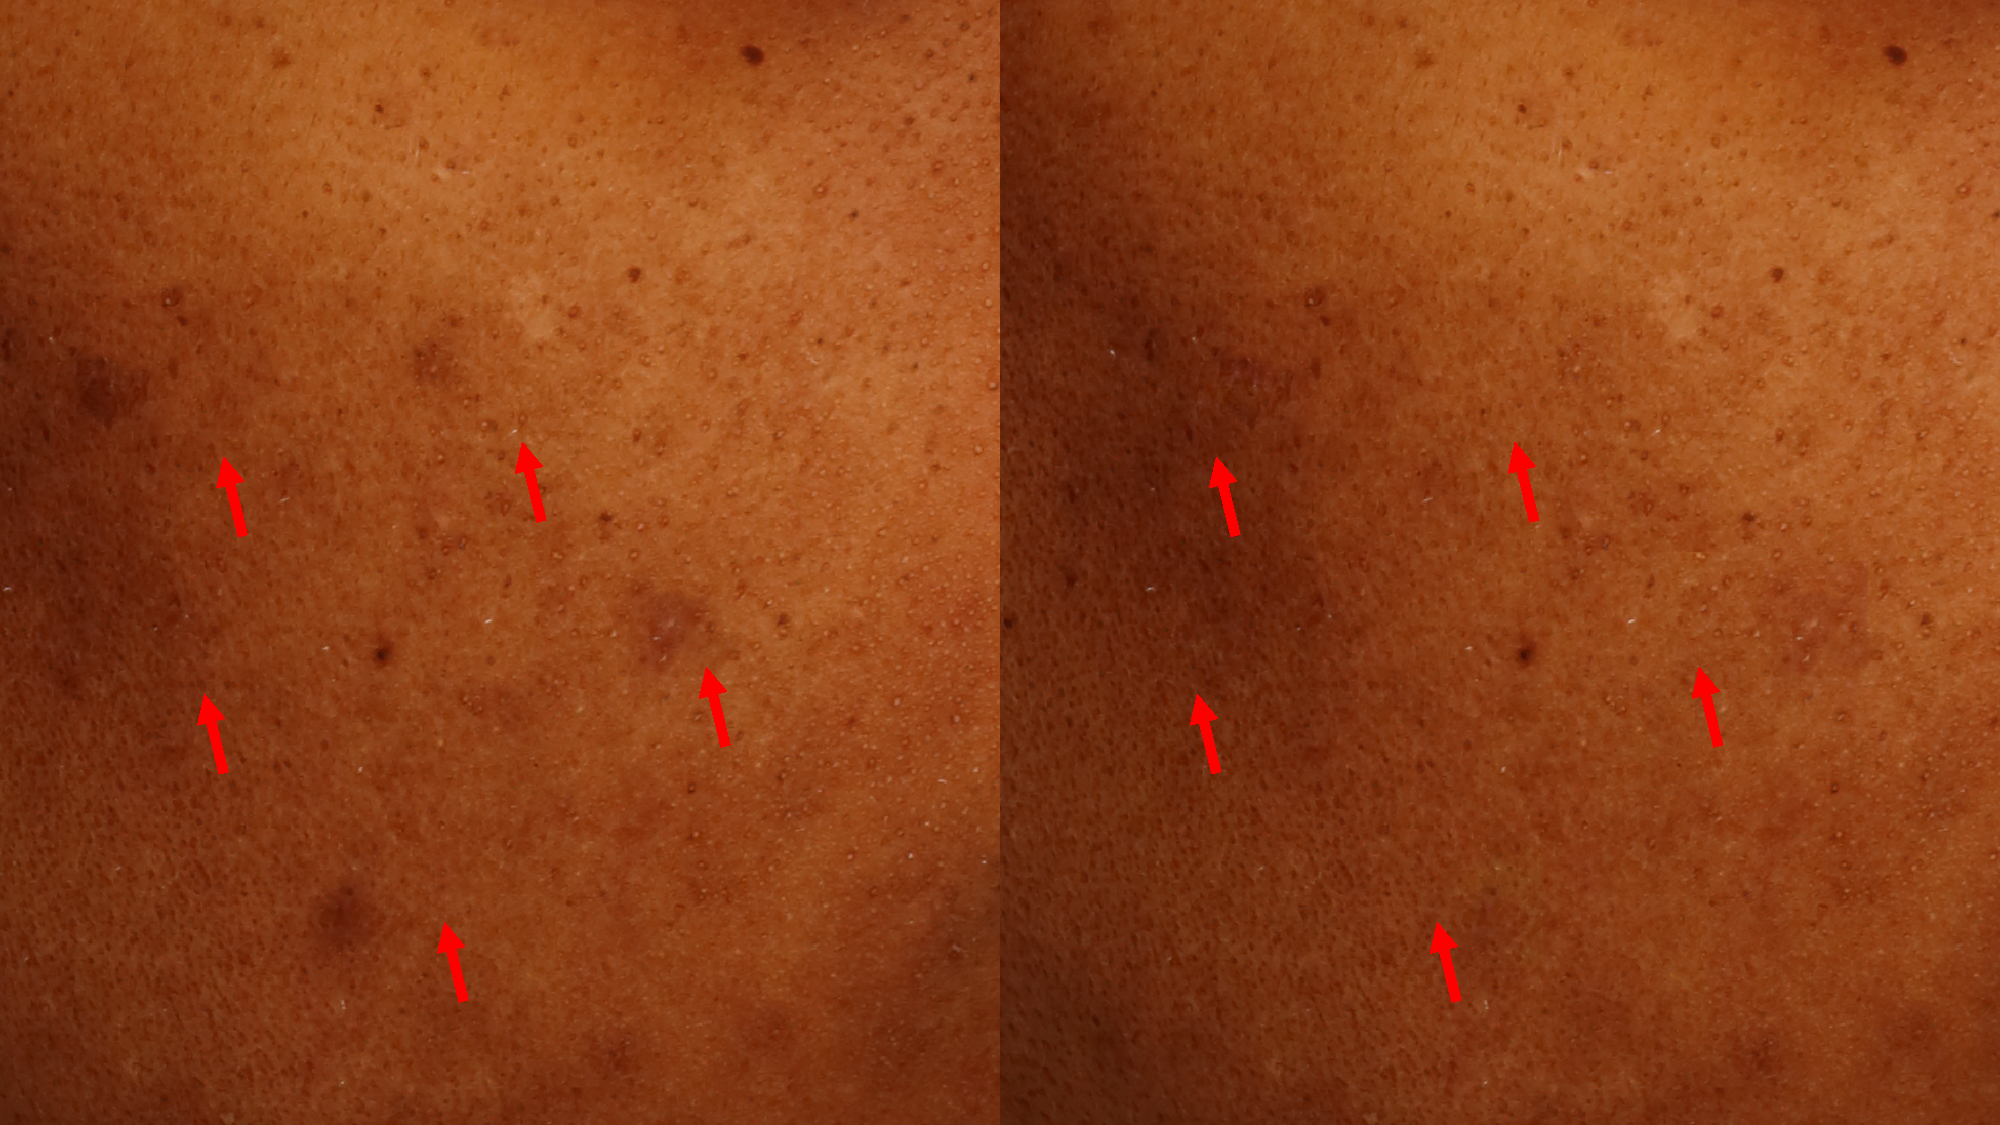
\includegraphics[width=.9\linewidth]{Appendix/img/2.pdf}
        \caption{Dark}
      \end{subfigure}
    \begin{subfigure}{.5\textwidth}
        \centering
        \includegraphics[width=.9\linewidth]{Appendix/img/3.pdf}
        \caption{Dark}
      \end{subfigure}%
      \begin{subfigure}{.5\textwidth}
        \centering
        \includegraphics[width=.9\linewidth]{Appendix/img/4.pdf}
        \caption{Dark}
      \end{subfigure}
    \begin{subfigure}{.5\textwidth}
        \centering
        \includegraphics[width=.9\linewidth]{Appendix/img/5.pdf}
        \caption{Brown}
      \end{subfigure}%
      \begin{subfigure}{.5\textwidth}
        \centering
        \includegraphics[width=.9\linewidth]{Appendix/img/6.pdf}
        \caption{Brown}
      \end{subfigure}
\end{figure}
\begin{figure}[p]\ContinuedFloat
    \begin{subfigure}{.5\textwidth}
        \centering
        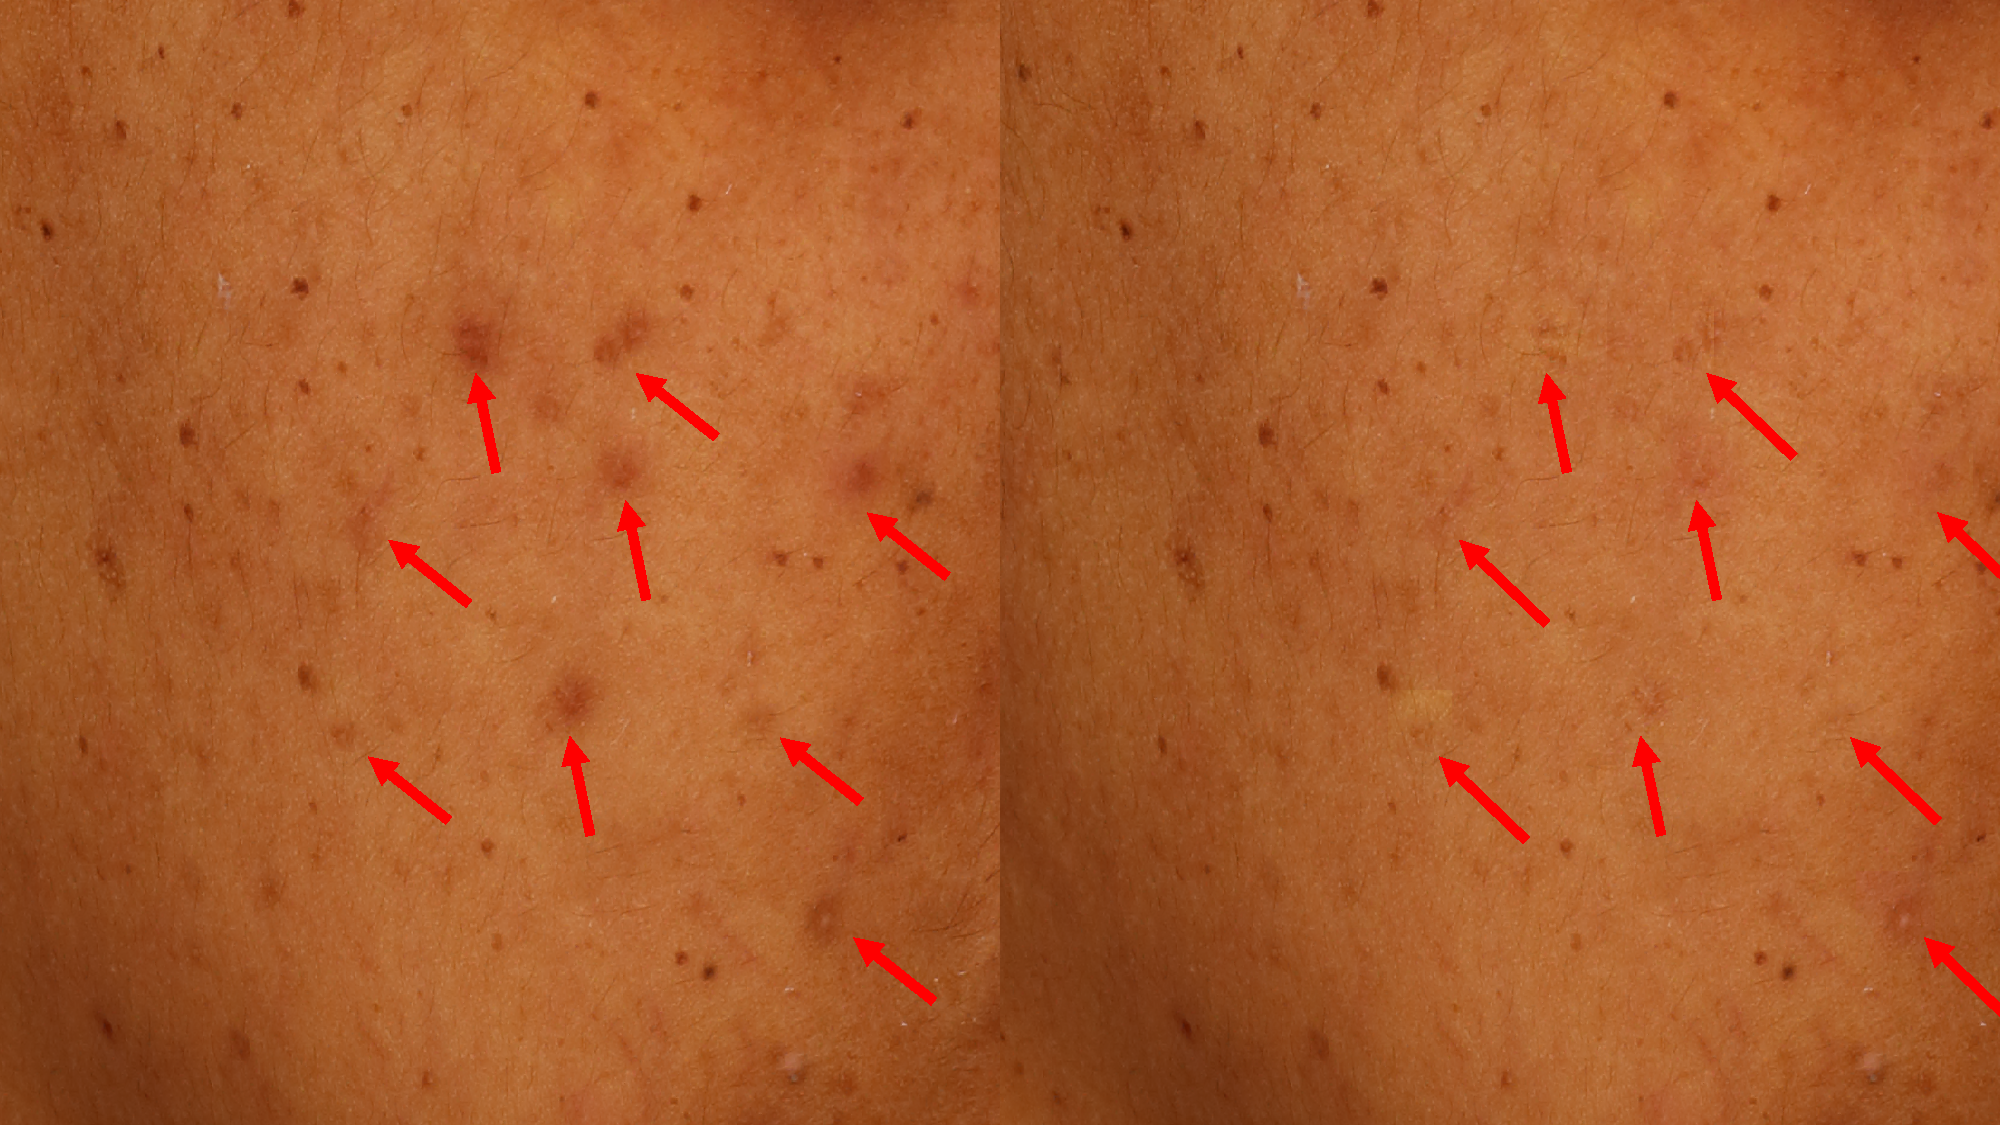
\includegraphics[width=.9\linewidth]{Appendix/img/7.pdf}
        \caption{Brown}
      \end{subfigure}%
      \begin{subfigure}{.5\textwidth}
        \centering
        \includegraphics[width=.9\linewidth]{Appendix/img/8.pdf}
        \caption{Brown}
      \end{subfigure}
    \begin{subfigure}{.5\textwidth}
        \centering
        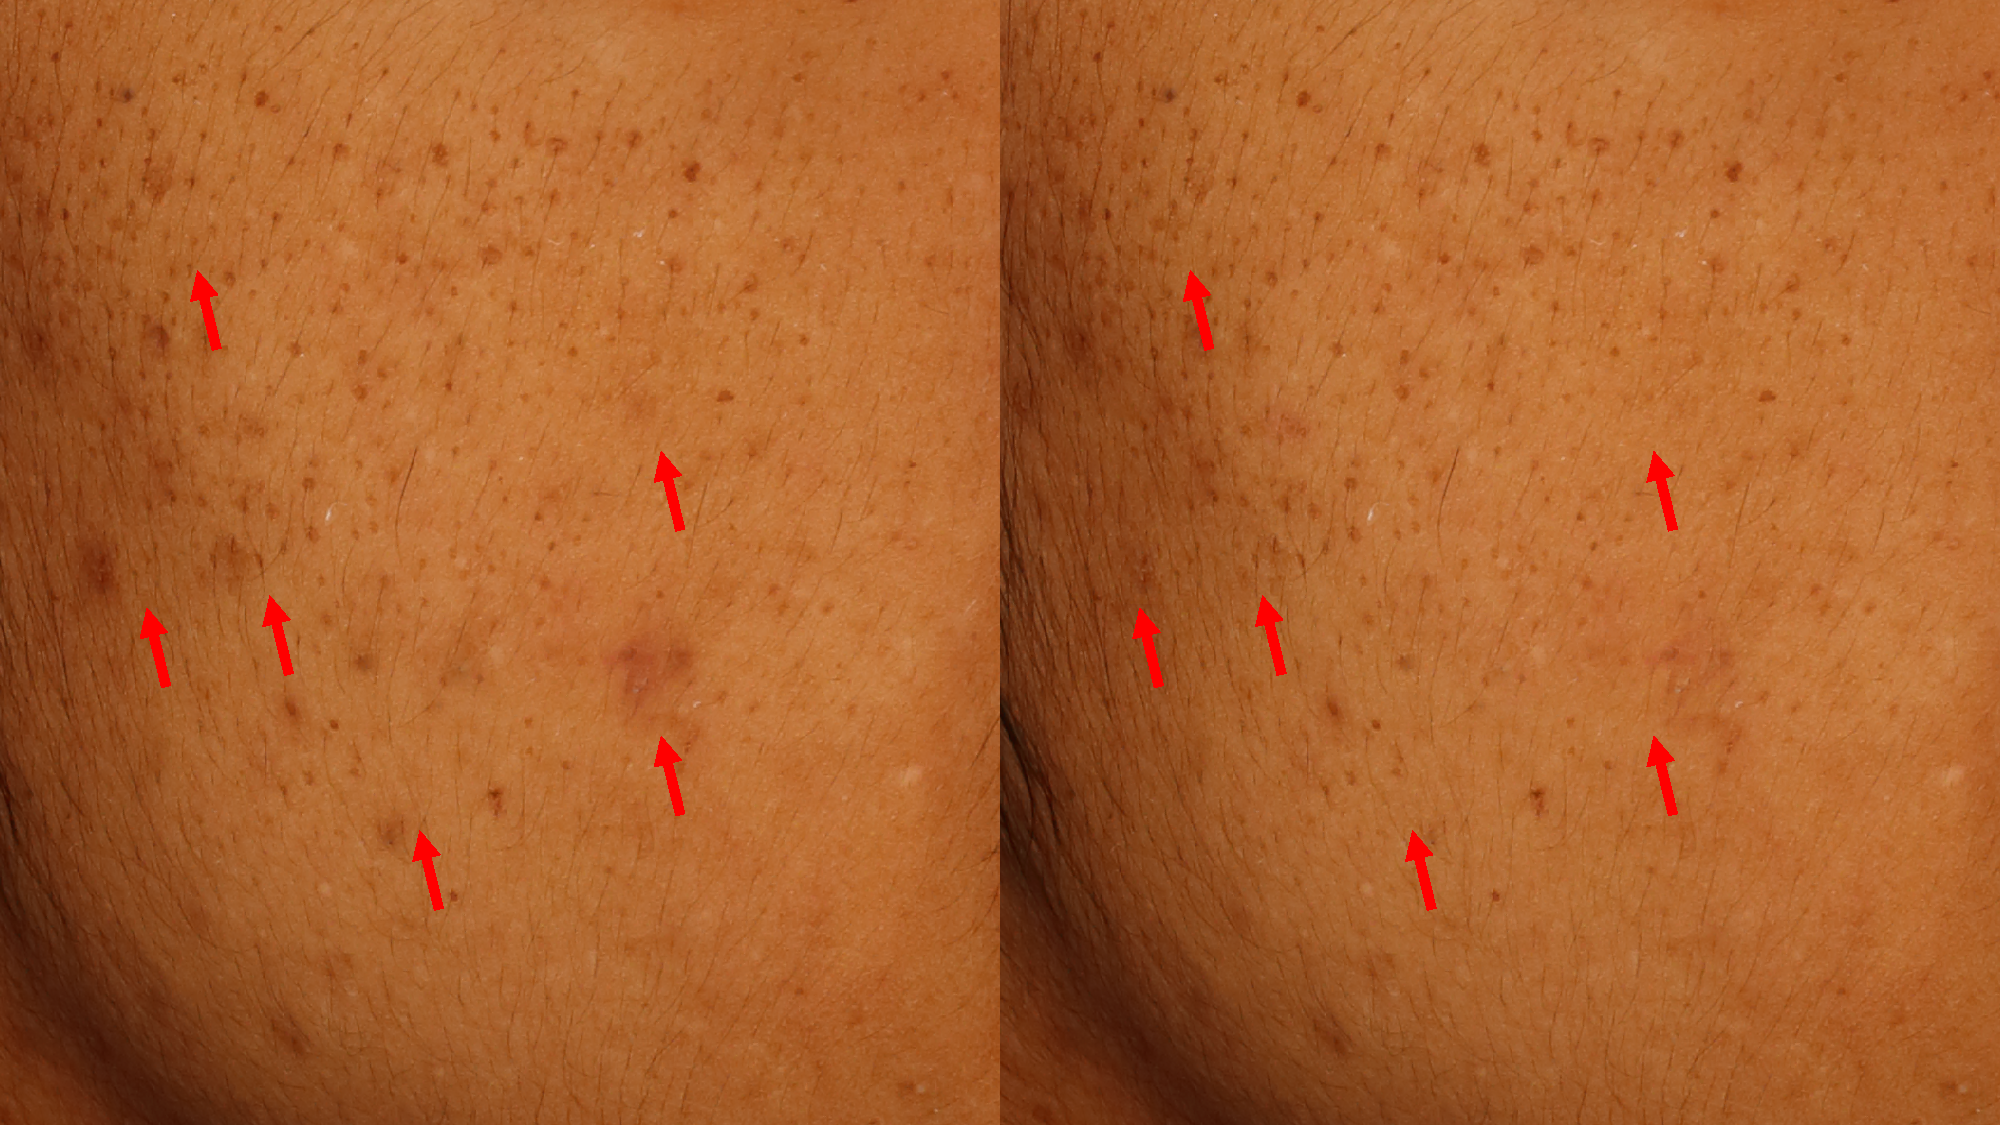
\includegraphics[width=.9\linewidth]{Appendix/img/9.pdf}
        \caption{Tan}
      \end{subfigure}%
      \begin{subfigure}{.5\textwidth}
        \centering
        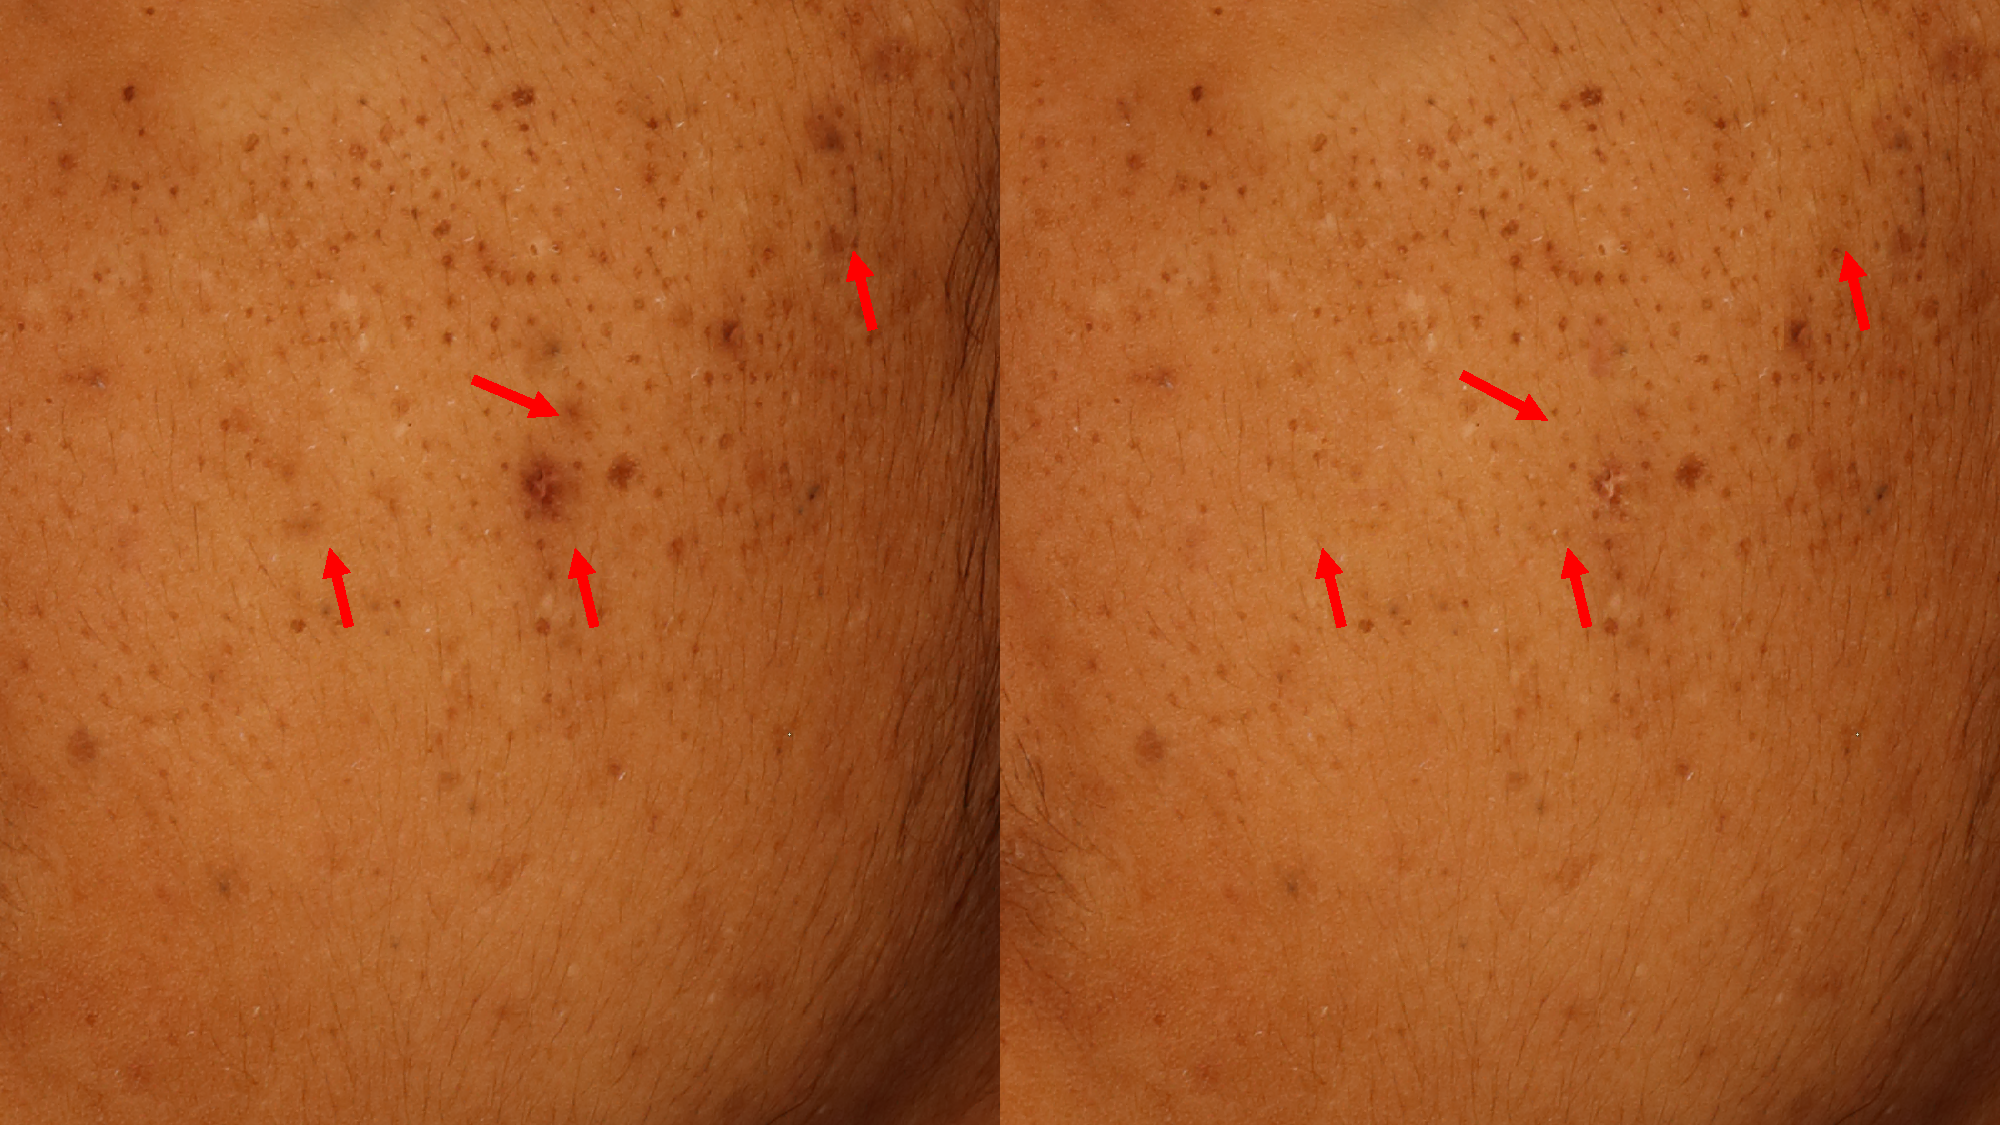
\includegraphics[width=.9\linewidth]{Appendix/img/10.pdf}
        \caption{Tan}
      \end{subfigure}
    \begin{subfigure}{.5\textwidth}
        \centering
        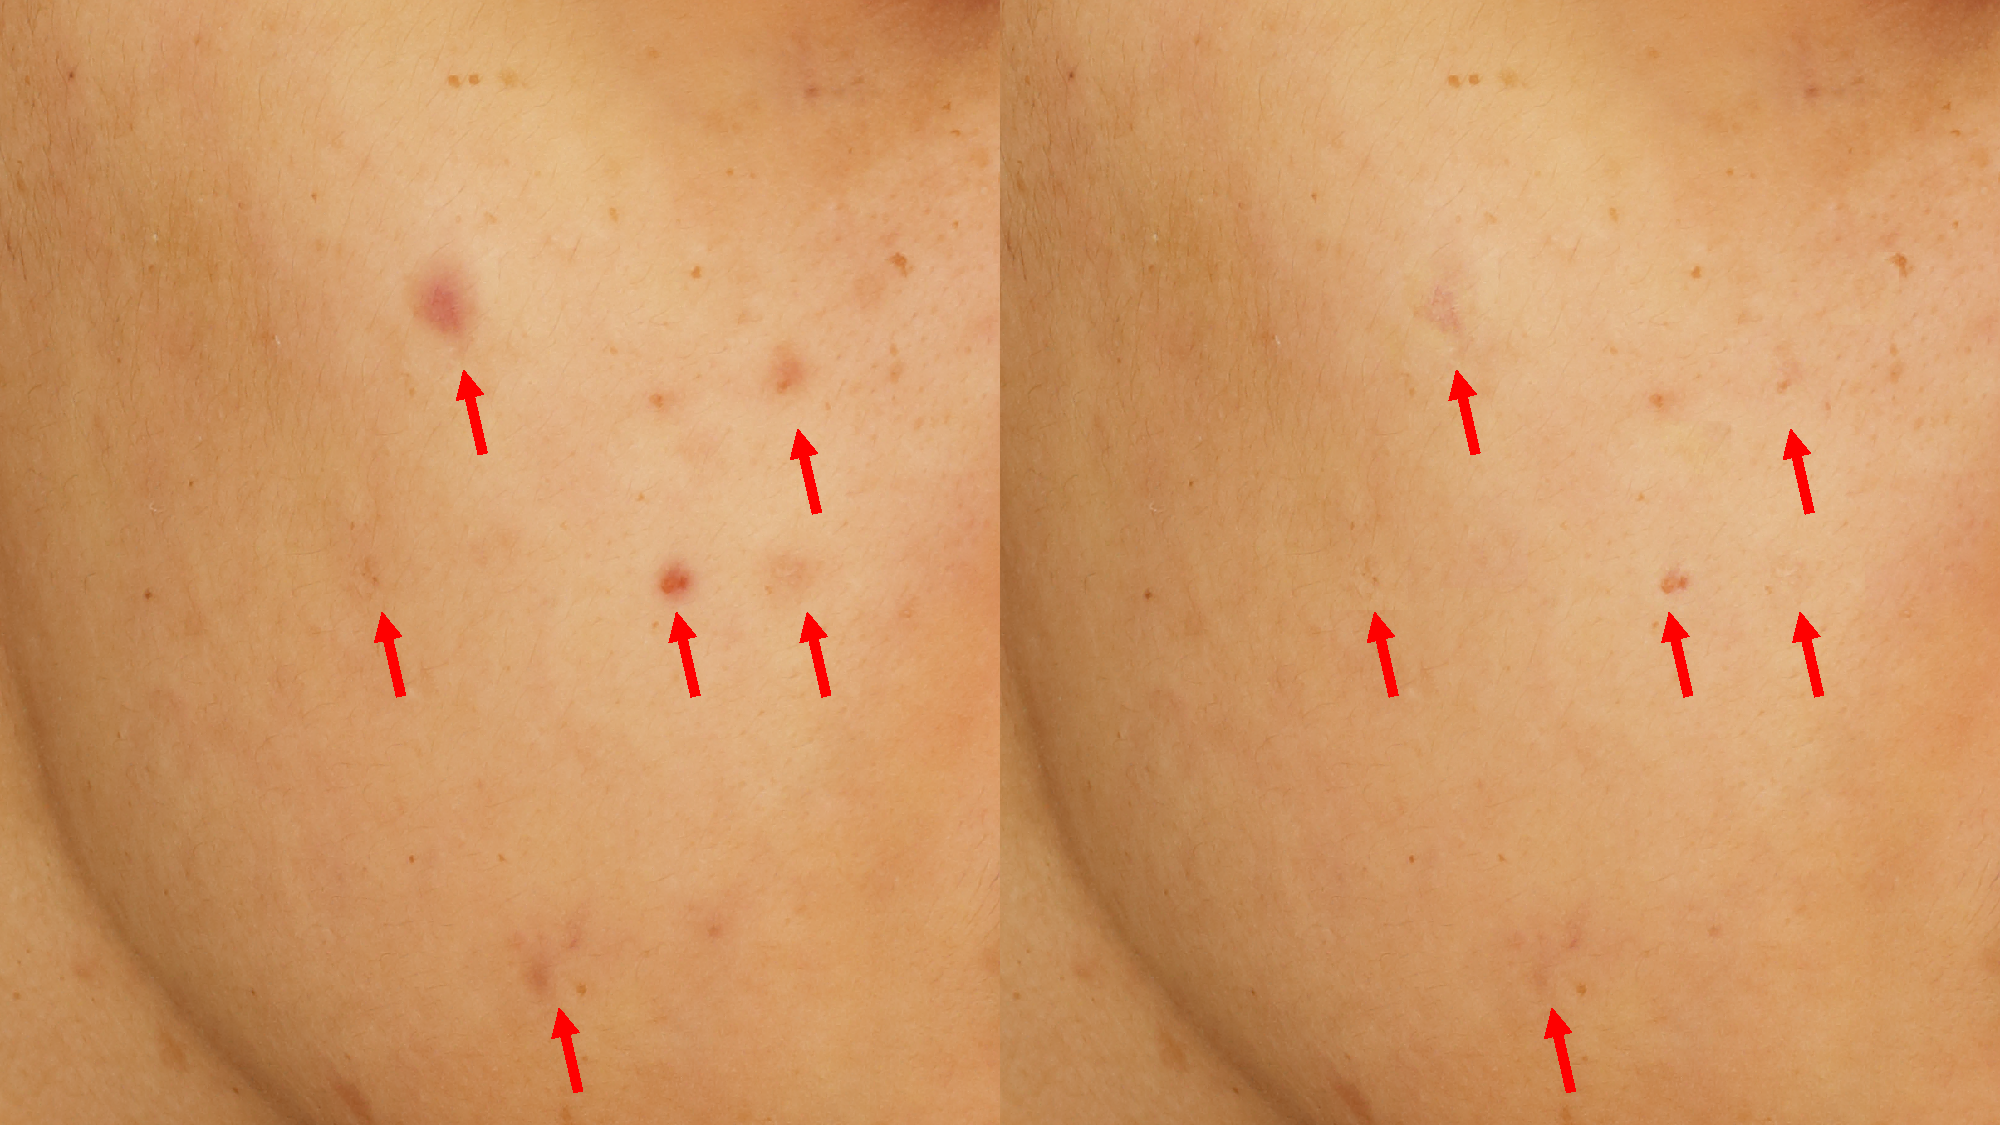
\includegraphics[width=.9\linewidth]{Appendix/img/11.pdf}
        \caption{Intermediate}
      \end{subfigure}%
      \begin{subfigure}{.5\textwidth}
        \centering
        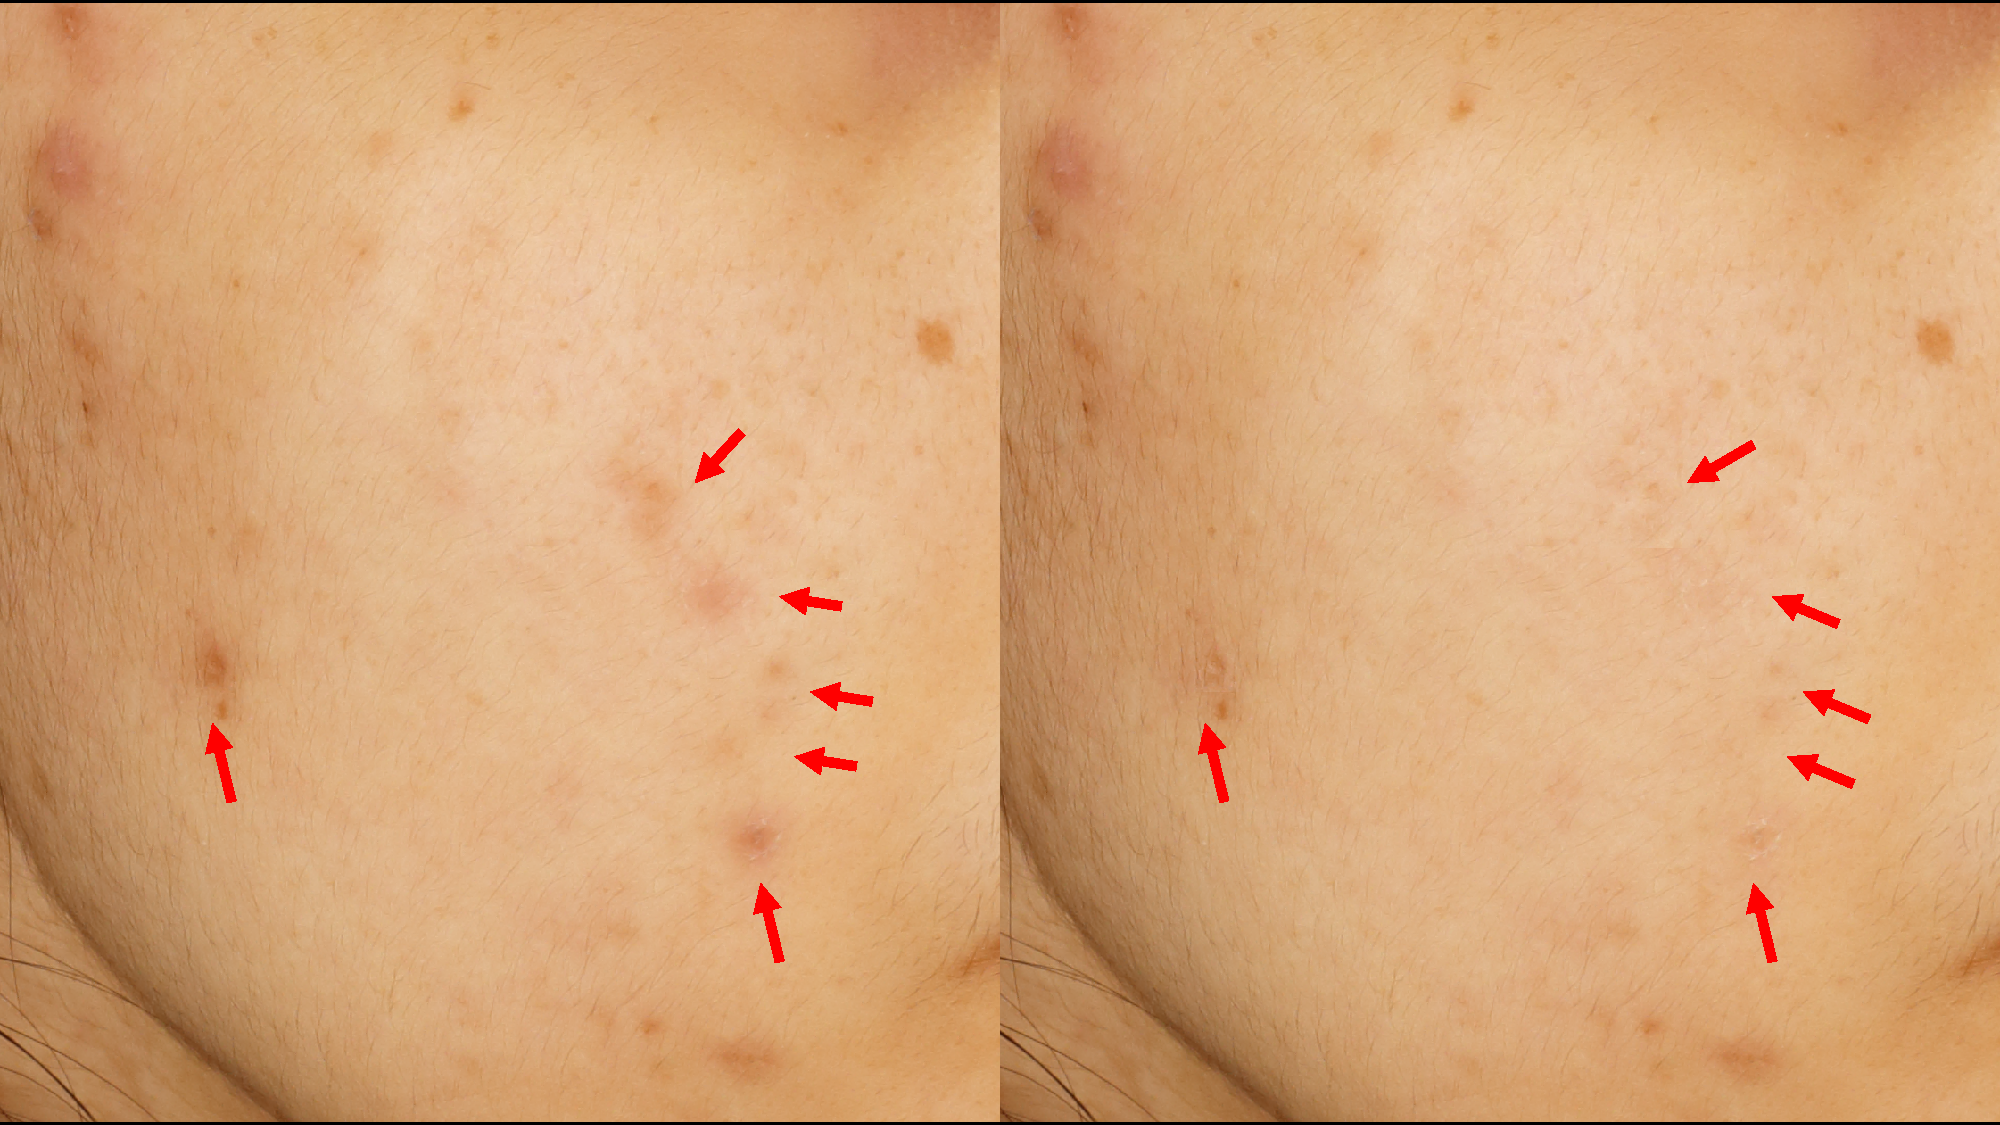
\includegraphics[width=.9\linewidth]{Appendix/img/12.pdf}
        \caption{Intermediate}
      \end{subfigure}
    \begin{subfigure}{.5\textwidth}
        \centering
        \includegraphics[width=.9\linewidth]{Appendix/img/13.pdf}
        \caption{Light}
      \end{subfigure}%
      \begin{subfigure}{.5\textwidth}
        \centering
        \includegraphics[width=.9\linewidth]{Appendix/img/14.pdf}
        \caption{Light}
      \end{subfigure}
    \begin{subfigure}{.5\textwidth}
        \centering
        \includegraphics[width=.9\linewidth]{Appendix/img/15.pdf}
        \caption{Light}
      \end{subfigure}%
      \begin{subfigure}{.5\textwidth}
        \centering
        \includegraphics[width=.9\linewidth]{Appendix/img/16.pdf}
        \caption{Light}
      \end{subfigure}
\end{figure}
\end{spacing}

% \chapter{Sample Code}
% \markboth{Appendix B}{} % For appendix second, etc.. 

% below shows how to insert highlighted source code from the source file.

% \inputminted[
% tabsize=4, % change this to set the spacing of tab
% breaklines, % automatically wrap the code
% fontsize=\scriptsize % Can be \footnotesize, \small, \normalsize etc
% ]{python}{Appendix/sample.py}

\end{appendices}